\usepackage{../common}

\title{Feature set analysis for chess \reflectbox{NNUE} networks}
\subtitle{Tesis de Licenciatura}
\author{Martín Emiliano Lombardo}
\institute{Departamento de Computación\\Facultad de Ciencias Exactas y Naturales\\Universidad de Buenos Aires}
\date{2024}
\titlegraphic{\includegraphics[height=1cm]{../assets/wN.pdf}}
\usetheme{Berlin}

%gets rid of bottom navigation bars
\setbeamertemplate{footline}[frame number]{}
%gets rid of bottom navigation symbols
\setbeamertemplate{navigation symbols}{}
%gets rid of footer
\setbeamertemplate{footline}{}

\begin{document}

\frame{\titlepage}

\section{Introduction}

% The rise of NNUEs
% https://stanford.edu/~cpiech/cs221/apps/deepBlue.html

% https://deepmind.google/discover/blog/alphazero-shedding-new-light-on-chess-shogi-and-go/
% https://crimsonpublishers.com/cojra/pdf/COJRA.000563.pdf
% https://arxiv.org/pdf/2209.11902.pdf

The development of chess engines was and continues to be a topic of study in the chess and computer communities for decades. IBM DeepBlue \cite{deepblue:2002} was the first chess machine to reach superhuman level by consistently beating the world champion, Garry Kasparov, in 1997 \cite{washingtonpost:1997}. Since then, engines have evolved in strength and complexity. \\

Chess can be modeled as a tree, where each node is a particular board configuration and the edges are legal moves for that position. With this representation, engines can use tree search algorithms to explore the tree and approximate the best move. Since the 1950s and to this date, engines have used algorithms like Minimax \cite{minimax-survey:1995} and Monte Carlo Tree Search \cite{mcts-survey:2012} (MCTS) or some of its variants \cite{tree-search-methods:2014,mcts-modifications:2022} to accomplish this.

The number of possible positions in chess is vast, estimated by Shannon \cite{shannon:1950} to be around $10^{43}$. This number is based on the average number of legal moves per position and the average game length. This makes it not feasible to explore the entire tree, so every tree search algorithm relies on having an evaluation function: a function that takes the state of the game and returns a single real number. This number is used to encompass information about the whole subtree of that position so it can be propagated up the tree, depending on the algorithm. Until a few years ago, highly complex handcrafted functions were used that were based on human knowledge about the game. \\

Until the 2010s, the development of engines advanced at a slow but consistent pace. Until 2017 that Google DeepMind published AlphaGo Zero \cite{alphagozero:2017} and its successor AlphaZero \cite{alphazero:2017,alphazero:2018} in 2018, which proved to be overwhelmingly superior (28 wins, 73 draws and 0 losses against the best engine at that time). They introduced a new approach to the development of board game engines, including chess: train a convolutional neural network with a reinforcement learning algorithm to learn to play by itself.

This change of paradigm, where the evaluation of positions is done by neural networks instead of functions built with human knowledge, altered the course of development of all modern engines (not just Go and chess). In 2018, Yu Nasu introduced the networks \reflectbox{EUNN} (or NNUE) ``Efficiently Updatable Neural-Networks'' \cite{nnue:2018} for the game Shogi. NNUE networks allow for cheap evaluations when evaluating a sequence of similar positions, making them ideal for use in depth-first search based engines. Since then, all modern engines have incorporated NNUE networks or some kind of neural network in their evaluation.

The chess engine Stockfish \cite{stockfish}, modern successor of DeepBlue with improved heuristics and running in commercial hardware is one of the strongest in the world. It incorporated NNUE networks mixed with classical evaluation in version 12\footnote[1]{\href{https://stockfishchess.org/blog/2020/introducing-nnue-evaluation/}{Introducing NNUE evaluation (Stockfish 12)}}. Since Stockfish 16.1\footnote[2]{\href{https://stockfishchess.org/blog/2024/stockfish-16-1/}{Removal of handcrafted evaluation (Stockfish 16.1)}} (2024) the evaluation is done exclusively through NNUE networks, eliminating all human aspect.

\newpage
\subsection{Thesis plan}

The main goal of this thesis is to explore different kinds of board encodings called feature sets. These encodings are the input for a NNUE network. To do so, I need a chess engine that supports neural networks with the ability to customize encodings and a way to train them.

I decided to implement a simple but capable classic engine based on well-known algorithms and optimizations, and then change the evaluation to use NNUE networks, with a versatile framework to build feature sets. Finally, I implemented a training pipeline to train the networks and measure their performance.

With the setup ready, I run multiple experiments. I propose different feature sets, train networks with them and compare their performance.

% The initial idea was to use Stockfish with the official Pytorch trainer \cite{nnue-pytorch}. However, I quickly realized that implementing some of the features sets I had in mind may be too complicated  with Stockfish's representation and the unconventional training test (PQR) that I wanted to do was impossible. This, and given that Stockfish engine and trainer codebases are huge, I felt there was too much magic involved so I turned away. I could have picked up another less complex engine written in Rust (like Marlin) and modify it, but I choose not to.
% So, I decided to implement my own engine and training pipeline from scratch.

\subsection{Source code}

The source code for this work can be found online in the following repositories:

\begin{table}[H]
\centering
\begin{tabular}{ll}
\toprule
\textbf{Repository} & \textbf{Repository} \\
\midrule
Source code & \url{https://github.com/mlomb/cs-master-thesis} \\
\LaTeX\ documents & \url{https://github.com/mlomb/cs-master-thesis-doc}
\end{tabular}
\end{table}


\section{Parte 1}

\subsection{Pepe}

\begin{frame}
\frametitle{Sample frame title}
This is some text in the first frame.\pause This is some text in the first frame. This is some text in the first frame.
\end{frame}

\begin{frame}
\frametitle{Sample frame title}

\begin{figure}[H]
\centering
\makebox[\textwidth]{\includegraphics[width=\textwidth]{../assets/sigmoid_fit.pdf}}
\caption{WDL model function (sigmoid) fitted to 100 million evaluations in the dataset.}
\label{wdl-fit}
\end{figure}

\end{frame}

\section{Parte 2}

\begin{frame}
\frametitle{Sample frame title}

\begin{figure}[H]
\centering
\makebox[\textwidth]{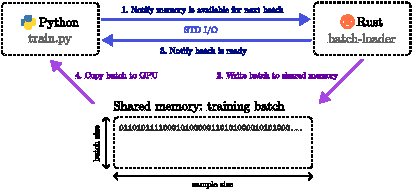
\includegraphics[width=\textwidth]{../assets/training-loop.pdf}}
\caption{Sequence of steps to send a batch from the \texttt{batch-loader} subprocess in Rust to Pytorch.}
\label{training-loop}
\end{figure}
\end{frame}


\begin{frame}
\frametitle{Sample frame title}
WORK IN PROGRESS
\end{frame}

\end{document}
